
In this lab we will perform social engineer.

Followin the instructions in the lab, I run the nc command on the IP and Port provided
that gives the following output.

\begin{figure}[H]
  \centering
  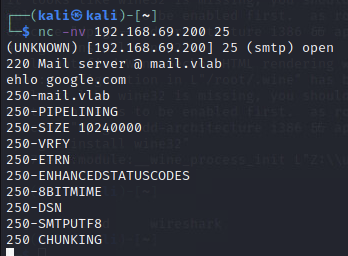
\includegraphics[width=0.5\textwidth]{figures/nc}
  \caption{Netcat output}
  \label{f:nc}
\end{figure}

We now have to enumerate a list of usernames provided. We will create a txt with
them.

\begin{figure}[H]
  \centering
  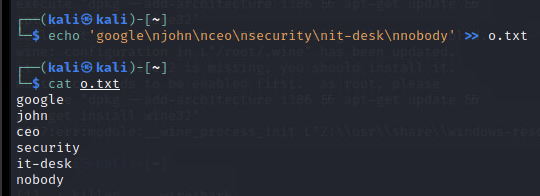
\includegraphics[width=0.5\textwidth]{figures/o}
  \caption{Text File with usernames}
  \label{f:o}
\end{figure}

We can now enumerate the SMTP with smtp-user-enum tool and the txt file
previously created.

\begin{figure}[H]
  \centering
  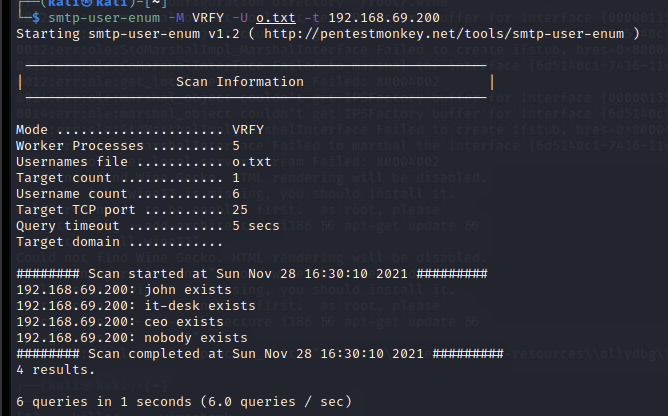
\includegraphics[width=0.6\textwidth]{figures/smtp-user-enum}
  \caption{Smtp-user-enum}
  \label{f:smtp-user-enum}
\end{figure}

Let's make sure we assign a sender and a recipient. Let's start with the sender.

\begin{figure}[H]
  \centering
  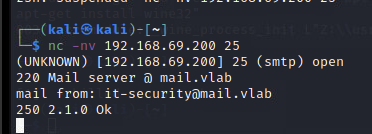
\includegraphics[width=0.6\textwidth]{figures/sender}
  \caption{sender}
  \label{f:sender}
\end{figure}

I made sure to use an email that has some kind of power such as the it-security
one. Impersonating the right person is very important for social engineering.

\begin{figure}[H]
  \centering
  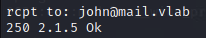
\includegraphics[width=0.6\textwidth]{figures/receiver}
  \caption{receiver}
  \label{f:receiver}
\end{figure}

We choose john as the receiver and we will now write an email to him, hoping that
he will get the bait and give us access to his machine remotely.

After failing with the previous set up I tried to look into more accounts as I realised
that the example from the task had Company IT Security in bold.
After tried to vrfy it-security following the format give from it-desk I found
that it was returning a positive message. This was probably one piece of the puzzle
that was missing.

\begin{figure}[H]
  \centering
  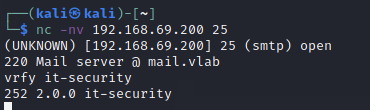
\includegraphics[width=0.5\textwidth]{figures/it-security}
  \caption{it-security}
  \label{f:it-security}
\end{figure}

Let's try again with a slightly different payload too.

\begin{figure}[H]
  \centering
  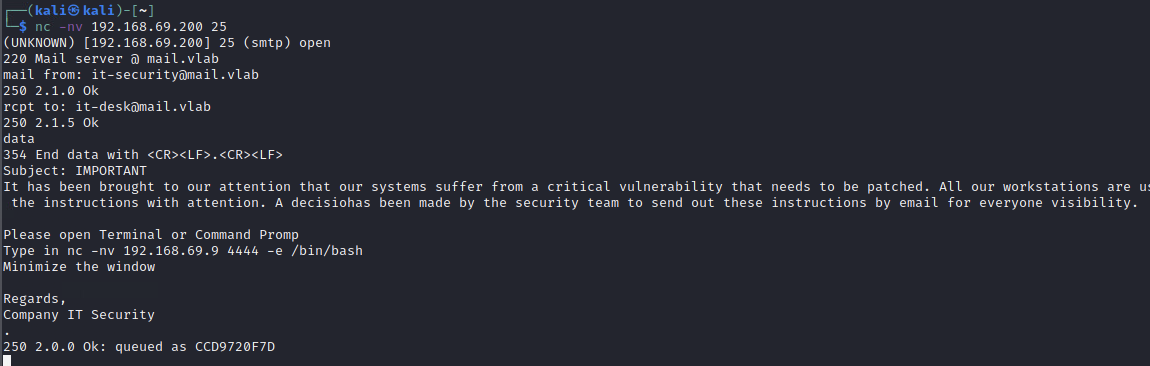
\includegraphics[width=1\textwidth]{figures/workingpayload}
  \caption{workingpayload}
  \label{f:workingpayload}
\end{figure}

Now let's hop on the other terminal that has been listening on the 4444 port
this whole time.

\begin{figure}[H]
  \centering
  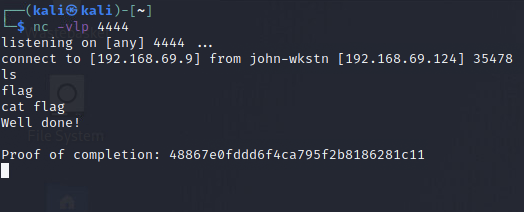
\includegraphics[width=1\textwidth]{figures/4444}
  \caption{4444}
  \label{f:4444}
\end{figure}

We have the flag!

\section{Conclusion}
This has been a very fun lab even though I got a bit frustrated by the typos I
was making in the email that made me lose a lot of time. This is an important
skill to have and we even see it in our lives everyday how social engineering is
being abused through emails.

